\documentclass[a4paper, 11pt]{article}

\usepackage{a4wide}
\usepackage{graphicx}
\usepackage{hyperref}
\usepackage{rotating}

\hypersetup{urlcolor=blue}

\setlength\parindent{0pt}

\title{Information Security Project}
\author{
Jan Vermeulen \and
Niels De Graef \and
Maxime Fern\'andez Alonso \and
Isaura Claeys
}

\begin{document}
\maketitle
\tableofcontents

\newpage

\section{Security services}
We will first discuss the required security services for the
vehicle-to-vehicle application. Afterwards we will elaborate in detail on
how these services protect the car/driver and how to achieve these
services.

\subsection{Data confidentiality}
Since the data exchanged between two vehicles might contain information such as
the state of the car, or possibly information regarding the driver of the
vehicle, we should regard the information exchanged as sensitive.
All the information exchanged between two vehicles should thus be confidential
and it should be impossible for a third entity to read by simply eavesdropping
on the communication channel.

\subsection{Authentication}
Since we are exchanging sensitive information with another entity, we want to
make sure the party on the other side is genuine and reliable. By this we mean
that we want to make sure that other party is not simply communicating to
exctract sensitive information, and that it does not have malicious intents.
Accepting information from an entity which has malicious intents could lead to
possible traffic problems. For this we need each entity to be identifiable and
authenticated. \\

Even though vehicles should be identifiable, it should not be possible
to track a certain vehicle, as well as link a vehicle to a specific
person.

\subsection{Data integrity}
Data integrity is also extremely important. We do not want data to be
altered by any party, otherwise it might provide wrong information and may
lead to car crashes or other traffic problems that may jeopardize drivers.
Since cars communicate directly with eachother, modifying data might be hard to
achieve. \\

We also do not want the logs to be modifiable in any way. Logs are the
equivalent of the black box in aircrafts.

\subsection{Non-repudiation}
It should not be able for a vehicle to deny it sent or received a certain
message. This is definitely important when an accident occurs or when a
certain vehicle is sending out wrong information, and we want to find out
the source of the problem. To achieve this, all data sent will be signed
by the sender and a signed acknowledgement will be sent back by the
receiver. We will also keep logs, which will contain sent and received
messages. To ensure data confidentiality, the logs can be encrypted using
a key given by the car manufacturer which will only ever be known by the car manufacturer.

\subsection{Availabilty}
The availability of the network is important, but not primordial. Correctly
operating vehicles should be wary of failing vehicles.
% Attackers might perform for example DoS attacks which overload the network
% and makes it impossible for vehicles to communicate with each other.
% When a vehicles leaves a platoon, it should send a leave message. When other
% vehicles notice a vehicle stops sending messages, without sending a
% leave-message, the other vehicles know they should be wary and take actions
% accordingly.

\section{Possible attacks}
% Against which attacks should these security services protect the system?
% Which countermeasures have been taken against these attacks?
% What are possible limitations and remaining vulnerabilities of your system?

\subsection{Eavesdropping}
If data confidentiality was not required, sensitive information could be
read by everyone by simply eavesdropping on the communication channel.
Simply encrypting the vehicle messages should solve this. This will be achieved
by using a symmetric key.

\subsection{Traffic Analysis}
Each session between two vehicles will be using a different symmetric key, which
will be exchanged using the Diffie-Hellmann key-exchangen algorithm. So within
the same session, limited information can be extracted from an encrypted stream.
However, as cars will be switching platoons quite frequently, this is not
considered a major issue.

\subsection{Message modification}
We should use a channel applying some form of encryption, as to make it
impossible to modify the content of the messages. Even though we already use
encryption, an attacker might still modify the encrypted data making the
original message unreadable.

\subsection{Replay}
A sequence number must be added to every form of communication between two
vehicles, as to make it impossible for an intruder to replay messages. When a
replay-attack is executed, the sequence number will be old and it will be
obvious that this is not a genuine message.

\subsection{Denial-of-Service} % Network DoS / Computational DoS
By overloading the connection between two vehicles (e.g. by flooding it
with packets), communicating becomes impossible. This problem cannot be
solved. \\

Another way to achieve a Denial-of-Service attack, is by targeting one specific
vehicle. If one continuously requests computationally expensive operations, the
vehicle might not be able to answer and refuse service. This can be solved by
caching results. % TODO -> wegvallen => graceful degradation

\subsection{Location tracking} Since every platoon is a local network,
tracking from outside this network is impossible. The most traceability that
can be done is that you can save a vehicle's public key, retrieved from a
Certification Authority, and you keep track of when you encounter that public
key again.

\subsection{Man-in-the-middle/hijacking} %taking over existing connection, where attacker replaces sender or receiver
Each pair of communicating cars uses a different symmetric key. This way
traffic cannot be hijacked, as the hijacker would need the key to be able
to send meaningful messages. All messages are also authenticated using the
private key of the other entity, making it impossible to impersonate that
entity.

\section{Security mechanisms}
%Which concrete security mechanisms (encryption algorithms, key lengths, etc.) do you use to implement these security services? Be sufficiently specific in the description of your choice.
The general idea consists of each car having a public and private key-pair that
is registered with a certification authority. After two cars exchange their
public keys, they set up a connection by exchanging a symmetric key. All
communication between the vehicles is now encrypted with this symmetric key. All public and
private key-pairs used in this project have been generated using Elliptic Curve
Cryptography (ECC) with 256 bits. Compared to RSA, ECC is faster and requires
less bits to achieve the same level of security.

\subsection{Certificate hierarchy}
Each vehicle has a certificate, signed by a trusted certification authority.
Every time the car is started, the public keys of the trusted CA's are fetched
and updated. This means the certificate of the car is kept in memory.
Another possibility is to have them hardcoded in the car's hardware.
This way we do not constantly need to ask the CA if the certificate of another car is
valid. Otherwise this would be quite time consuming, which would not benefit our
hard time limit. Whenever a car is brought in for maintenance the certificate of
the car can be renewed.\\

Obviously, one root authority signing the certificates of each car might not be the best solution.
This is why a hierarchy should be built that chains a root CA to car manufacturers and maybe even garages.

\subsection{Key exchange}
When a car joins a platoon, a secure communication session should be
established. This is achieved using the Elliptic Curve Diffie-Hellman Ephemeral
(ECDHE) key-exchange mechanism, which ensures that a shared secret key is
exchanged between two parties, assuming an insecure communication channel. We
opted to use Ephemeral Diffie-Hellman to provide forward secrecy. This means we
generate a new Diffie-Hellman key-pair every time we set up a connection. We use
the \texttt{SECP256R1} curves with a key-size of 256 bits. The other choice is
Diffie-Hellman using RSA with 2048-bit keys but as ECDH uses less bits and is
faster, this was the obvious choice. When sending the message containing our DH
public key, we sign it using our private key.
The associated public key is then used to verify this signature,
which is registered with the CA, to provide authentication.
This way we are sure that we are establishing a shared key
with the right entity.\\

Figure 1 shows a structured overview of the key exchange process.

\newpage
\subsection{Encryption channel}
The shared key we create during the DH key-exchange will be used as a symmetric
key in a AES-128 encrypted communication channel.
We opt for symmetric encryption because asymmetric encryption is a lot slower. This again does not benefit
our hard time limit.
Using a 128 bit symmetric key is sufficiently secure in this case. We use the
GCM (authenticated) mode to provide authentication and integrity. Using this
mode, we can check whether a message has been modified in any way. We opted to
use this mode for its functionality and because it is quite fast, as well as
parallelizable.\\

Figure 2 shows a structured overview of the necessary steps to send a message.

% ECDHE figuur uitleg
\begin{sidewaysfigure}[ht]
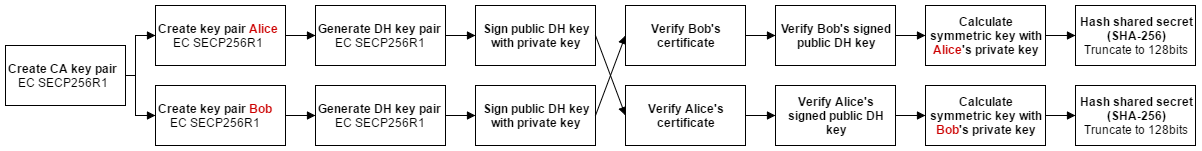
\includegraphics[scale=0.5]{imgs/IS_Demo_DH}
\caption{Communication initialization schematic}
\end{sidewaysfigure}

\begin{sidewaysfigure}[ht]
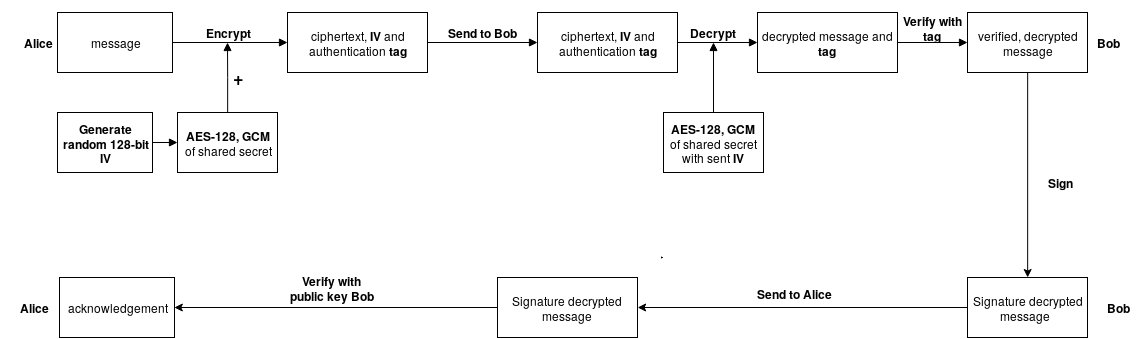
\includegraphics[scale=0.5]{imgs/IS_Demo_MSG}
\caption{Messaging schematic}
\end{sidewaysfigure}

\subsection{Graceful degradation}
When the secure communication channel is set up correctly, each pair of vehicles exchanges a message
at regular intervals (for example, every 10ms), to ensure driving safety. When a message is not received for two
intervals, cars should keep more distance from the vehicle in question.
Using this communication schema, a car can drive away from the platoon whenever it wishes.
When a car increases its distance to the platoon, communication channels will start failing and other cars will consider it to have left the platoon automatically.


\section{Remaining vulnerabilities}
The network is still the weakest point. If a signal jammer is mounted
on one of the vehicles, there is nothing that can be done to remove the
noise from the electro-magnetic field near the platoon. \\

Also, as we are using an ad-hoc network, this means it is effectively impossible to mitigate a denial-of-service
attack.

\section{Demo}
We constructed our demo application using Python $2.7$ and used the Cryptography
\footnote{https://cryptography.io/en/latest/} library for all cryptographic
functionality. To start the demo, just execute \texttt{main.py}.\\

The \texttt{certificates.py} file contains all the code to generate the static
certificates and mimic a CA. For the purpose of this demo, the CA we use is not
an external CA, but merely a key-pair that is used to sign each certificate of
the cars involved. It is also not part of a hierarchy.\\

\texttt{Person.py} contains the necessary functions for communication setup and
normal communication. This includes elliptic curve key generation (as we use
Ephemeral DH), as well as Diffie-Hellman key exchange, encryption, decryption
and signing methods.\\

\texttt{Main.py} will check if initial certificates are present and call
\texttt{certificates.create\_certificates()} if negative. Then it will create
two instances of \texttt{person.py}, namely Alice and Bob, and initiate their
communication. Then, a sample message and acknowledgement is sent and
communication is terminated. Some timer information is also measured and
printed, to be able to estimate the practical use of our vehicle-to-vehicle
communication.\\

A run on 2,3 GHz Intel Core i7 processor shows us that the communication setup
takes 2.61 ms. Sending a message takes 0.81 ms. This obviously does not include
network delay as we are simulating communication on a single piece of hardware.
These delays are acceptable within the real-time constraints of
vehicle-to-vehicle communication.


% figure that illustrates our demo code

\section{Conclusion}
Using the right cryptographic algorithms, it is possible to implement a secure
vehicle-to-vehicle communication. However, as this communication will use the
wireless medium, the network will always remain a vulnerability. It will never
be possible to prevent malicious users from jamming the medium or executing a
DOS attack. Aside from this limitation, the current state of the art technology
permits such communication to be implemented securely into smart cars. The main
difficulty that car manufacturers should overcome at this point is to agree on a
general standard for this kind of communication. This will only be a matter of time and effort.

\section{Sources}
\begin{itemize}
  \item \href{http://orff.uc3m.es/bitstream/handle/10016/9395/Overview-VANET-security-issues-earchivo.pdf?sequence=1}{Overview of security issues in Vehicular ad-hoc networks}
  \item \href{https://crypto.stackexchange.com}{Cryptography StackExchange}
  \item \href{https://security.stackexchange.com}{Security StackExchange}
\end{itemize}


\end{document}
